% ============================================================
%  物联网技术与实践 — 第 2 次 STM32 实验报告
%  编译: xelatex hw.tex
% ============================================================
\documentclass[a4paper,12pt,fontset=windows]{ctexart}

% ---------- 页面布局 ----------
\usepackage[top=2.54cm, bottom=2.54cm, left=3.17cm, right=3.17cm]{geometry}

% ---------- 图形 & 表格支持 ----------
\usepackage{graphicx}
\usepackage{float}
\usepackage{array}
\usepackage{tabularx}
\usepackage{booktabs}
\usepackage{caption}
\usepackage{tikz}
\usepackage{tikzpagenodes}

% ---------- 代码 ----------
\usepackage{listings}
\usepackage{xcolor}

% ---------- 超链接 ----------
\usepackage[colorlinks=true,linkcolor=black,urlcolor=blue]{hyperref}

% ---------- 自定义格式 ----------
\usepackage{titlesec}
\usepackage{enumitem}
\usepackage{indentfirst}

\pagestyle{plain}
\setlength{\parindent}{2\ccwd}
\setlength{\parskip}{0pt}
\linespread{1.25}
\setlist[itemize]{itemsep=2pt,topsep=2pt}
\setlist[enumerate]{itemsep=4pt,topsep=4pt}
\captionsetup{font=small,labelfont=bf}
\setcounter{secnumdepth}{1}
\renewcommand{\thesection}{\chinese{section}}
\titleformat{\section}[block]{\heiti\bfseries}{\thesection、}{0em}{}
\titleformat{\subsection}[block]{\bfseries}{}{0em}{}
\titleformat{\subsubsection}[block]{\bfseries}{}{0em}{}
\titlespacing*{\section}{0pt}{0.8em}{0.5em}
\titlespacing*{\subsection}{0pt}{0.6em}{0.4em}
\titlespacing*{\subsubsection}{0pt}{0.5em}{0.3em}

% ---------- 整页外框 ----------
\AddToHook{shipout/background}{%
  \begin{tikzpicture}[remember picture,overlay]
    \draw[line width=0.8pt]
      ([xshift=-10pt,yshift=10pt]current page text area.north west)
      rectangle
      ([xshift=10pt,yshift=-10pt]current page text area.south east);
  \end{tikzpicture}%
}

% ---------- 代码样式 ----------
\lstset{
  language=C,
  basicstyle=\small\ttfamily,
  keywordstyle=\color{blue},
  commentstyle=\color{gray},
  stringstyle=\color{red!70!black},
  numbers=left,
  numberstyle=\tiny\color{gray},
  numbersep=5pt,
  frame=single,
  breaklines=true,
  tabsize=2,
  showstringspaces=false,
  captionpos=b,
  xleftmargin=2em,
  framexleftmargin=1.5em,
  escapeinside={(*@}{@*)},
  extendedchars=true,
  inputencoding=utf8,
}

% ---------- 快捷命令 ----------
\newcommand{\coverentry}[1]{\makebox[8.6cm][c]{\underline{\makebox[7.6cm][c]{#1}}}}
\newcommand{\insertfigure}[3]{%
  \begin{figure}[H]
    \centering
    \includegraphics[width=#1\textwidth]{figs/#2}
    \caption{#3}
    \label{fig:#2}
  \end{figure}
}

\begin{document}
\zihao{-4}

% ========== 封面 ==========
\thispagestyle{empty}
\begin{center}
  \vspace*{2.8cm}

  {\zihao{-2}\heiti\bfseries 《物联网技术与实践》实验报告}

  \vspace{2.2cm}

  {\renewcommand{\arraystretch}{1.9}
  \begin{tabular}{@{}>{\centering\arraybackslash}m{2.8cm}>{\centering\arraybackslash}m{8.8cm}@{}}
    \zihao{4}\bfseries 年级： & \coverentry{2023级} \\[0.9cm]
    \zihao{4}\bfseries 专业： & \coverentry{电子信息科学与技术} \\[0.9cm]
    \zihao{4}\bfseries 姓名： & \coverentry{邵逸帆} \\[0.9cm]       % TODO: 填写姓名
    \zihao{4}\bfseries 学号： & \coverentry{320230900621}         % TODO: 填写学号
  \end{tabular}}
\end{center}
\newpage

% ========== 正文 ==========
\begin{center}
  {\heiti\zihao{3}\bfseries 基于STM32F070CBT6TR+HT7017的直流电能表开发板实验}
\end{center}

\section{实验目的}

\begin{sloppypar}
本实验旨在掌握基于 STM32CubeMX 与 CLion 的嵌入式开发流程，熟悉 STM32F070CBT6TR 开发板的使用。通过实验理解并掌握 GPIO、定时器、外部中断等外设的配置方法，掌握有限状态机（FSM）在嵌入式系统中的应用。同时学习 GN1650 数码管驱动芯片与 HT7017 直流计量芯片的工作原理，掌握 UART、I2C 通信协议及外设 API 的调用方法。此外，了解 RS485 半双工通信原理及 HC-05 蓝牙模块的使用方法，实现开发板与上位机或手机端的数据交换，培养硬件连接、代码烧录、串口通信调试及系统联调等综合调试能力。
\end{sloppypar}

\section{实验设备与环境}

硬件方面，使用基于 STM32F070CBT6TR + HT7017 的直流电能表开发板，配合 SEGGER J-Link 调试器、``野火小智''串口模块、CH340(HW597) 串口模块、HC-05 蓝牙模块、面包板和杜邦线等。软件方面，开发环境为 Windows 10/11 + CLion + STM32CubeMX + STM32CubeCLT，调试工具包括 OpenOCD 与 J-Link 驱动、串口调试助手 XCOM 以及 HC 蓝牙助手 APP。

\section{实验内容}

\subsection*{实验原理}

本实验基于 STM32F070CBT6TR 微控制器（Cortex-M0 内核，48\,MHz 主频，64\,KB Flash，8\,KB RAM），配合 HT7017 直流计量芯片，实现红绿灯控制、模拟电梯和直流电表数据采集三个功能模块。

\begin{sloppypar}
三个模块的核心设计思想是有限状态机（FSM）与中断驱动架构。红绿灯和电梯系统均将状态切换逻辑集中在定时器中断回调 \texttt{HAL\_TIM\_PeriodElapsedCallback} 中，主循环仅负责数码管刷新和 LED 更新，从而实现逻辑与显示的分离。按键事件通过外部中断回调 \texttt{HAL\_GPIO\_EXTI\_Callback} 处理，避免了轮询方式对 CPU 资源的浪费。
\end{sloppypar}

外设通信方面，GPIO 驱动红/绿/黄三色 LED 指示系统状态；TIM6 配置为 2\,Hz 周期中断（500\,ms 定时），作为系统心跳驱动倒计时和楼层移动；TIM15 以 PWM 模式驱动无源蜂鸣器，通过调节自动重装载寄存器（ARR）改变输出频率。数码管显示采用 bit-bang 模拟 I2C 协议驱动 3 组 GN1650 芯片，每组 4 位数码管。HT7017 计量芯片通过 USART1（4800\,bps、9 位数据位、奇校验）与 MCU 通信，RS485 半双工总线（USART4，38400\,bps）用于向上位机发送采样数据。

\subsection*{硬件连接与组装}

开发板主要外设引脚分配如表~\ref{tab:pins} 所示。硬件连接时，将 J-Link 调试器通过 SWD 接口连接开发板进行程序烧录与调试；RS485 通信链路为开发板 PCB 接入 ``野火小智'' 模块，再由该模块接入 CH340(HW597) 串口模块并连接 PC。该链路中，``野火小智'' 与 CH340(HW597) 采用串口直连方式连接，即 TX 对 TX、RX 对 RX。相比之下，HC-05 蓝牙模块接线采用 TX 对 RX、RX 对 TX 的交叉连接方式。

\begin{table}[H]
\centering
\caption{主要外设引脚分配}\label{tab:pins}
\small
\begin{tabularx}{\textwidth}{llX}
\toprule
\textbf{外设} & \textbf{引脚} & \textbf{说明} \\
\midrule
红色 LED  & PB1  & 高电平点亮 \\
绿色 LED  & PB0  & 高电平点亮 \\
黄色 LED  & PA7  & 高电平点亮 \\
测试 LED  & PA11 & 低电平点亮 \\
蜂鸣器    & PA2  & TIM15\_CH1 PWM 输出 \\
按键      & PB4/PA15/PB3/PB5 & EXTI 中断，低电平触发 \\
数码管    & 模拟 I2C & 3 组 GN1650，开漏输出 \\
HT7017   & PA9(TX)/PA10(RX) & USART1, 4800-9-Odd \\
RS485    & PA0(TX)/PA1(RX)  & USART4, 38400-8-None \\
\bottomrule
\end{tabularx}
\end{table}

% TODO: 取消注释并替换为实际硬件连接照片路径
% \insertfigure{0.70}{hardware.jpg}{硬件连接实物图}

\subsection*{软件设计与代码实现}

\subsubsection*{1. 红绿灯控制系统}

红绿灯系统采用 FSM 设计，定义了运行、设置红灯时长、设置绿灯时长三个系统模式，以及红灯和绿灯两个灯状态。运行模式下红绿灯按预设时长自动倒计时切换，数码管 1 显示当前倒计时，数码管 2、3 分别显示红灯和绿灯的设定时长，红灯期间蜂鸣器同步鸣叫。按键交互方面，RIGHT 键循环切换模式，UP/DOWN 键调整时长（5--99 秒），LEFT 键保存并返回运行模式，编辑中的数码管以 1\,Hz 闪烁提示。

TIM6 每 500\,ms 触发一次中断，每两次中断（1 秒）递减倒计时，归零时自动切换灯状态。关键实现如下：

\begin{lstlisting}
void HAL_TIM_PeriodElapsedCallback(TIM_HandleTypeDef *htim) {
  if (htim->Instance == TIM6) {
    timer_ticks++;
    g_flash_state = !g_flash_state; // (*@每 500 ms 翻转一次，用于数码管闪烁@*)
    // (*@运行模式下每 2 个 tick（1 s）递减一次倒计时@*)
    if (timer_ticks % 2 == 0 && g_system_mode == MODE_RUNNING) {
      if (g_current_countdown > 0) {
        g_current_countdown--;
      } else { // (*@倒计时归零后切换红绿灯状态@*)
        if (g_current_state == STATE_RED) {
          g_current_state = STATE_GREEN;
          g_current_countdown = g_config_green_duration;
        } else {
          g_current_state = STATE_RED;
          g_current_countdown = g_config_red_duration;
        }
      }
    }
  }
}
\end{lstlisting}

\subsubsection*{2. 模拟电梯系统}

\begin{sloppypar}
电梯系统采用 8 状态 FSM，由 TIM6 中断驱动楼层移动，实现完全非阻塞设计。上电后处于 1 楼待机（\texttt{STATE\_IDLE}），用户按 RIGHT 键依次进入选择起始楼层和目标楼层状态，选择时数码管闪烁提示。确认后电梯运行至接客楼层（红灯亮），到达后开门等待 3 秒（黄灯亮、蜂鸣器短鸣），再前往目标楼层（绿灯亮），最后自动返回 1 楼。
\end{sloppypar}

移动逻辑在定时器中断中实现，每次中断楼层加减 1，到达目标后自动切换状态：

\begin{lstlisting}
case STATE_MOVING_TO_USER:
  // (*@每个时基周期向用户所在楼层移动一层@*)
  if (g_elevator_current_floor < g_user_selected_floor)
    g_elevator_current_floor++;
  else if (g_elevator_current_floor > g_user_selected_floor)
    g_elevator_current_floor--;
  else { // (*@到达接客楼层后切换到开门等待状态@*)
    g_system_state = STATE_DOOR_OPEN_USER;
    g_wait_counter = DOOR_WAIT_SECONDS; // (*@开门保持 3 秒@*)
    Buzzer_On(); // (*@到达提示音@*)
  }
  break;
\end{lstlisting}

\subsubsection*{3. 直流电表数据采集}

\begin{sloppypar}
HT7017 计量芯片通过 USART1（4800\,bps、9 位数据、奇校验）与 MCU 通信。通信协议基于帧格式：帧头 0xA5、命令字节、数据字节和校验和（前述字节之和取反）。初始化时需先开启写保护，再向 ADCCON 寄存器（59H）写入配置值启动计量。TIM6 中断中周期调用 \texttt{HT7017\_GetSignedSample()} 读取电压、电流和功率的 24 位有符号原始值，经符号扩展后在主循环中通过数码管显示并经 RS485 发送至上位机。由于实验环境无 24\,V 外部负载，电表模块仅完成通信验证和裸数据采集。
\end{sloppypar}

\begin{lstlisting}
// (*@在定时路径中周期采集电压和电流原始值@*)
HT7017_GetSignedSample(&h_ht7017,
  HT7017_REG_SPL_U, (int32_t *)&g_raw_voltage);
HT7017_GetSignedSample(&h_ht7017,
  HT7017_REG_SPL_I1, (int32_t *)&g_raw_current);

// (*@在主循环中显示采样值，并通过 RS485 上报@*)
displayInteger(DISP_VOLTAGE, (int)g_raw_voltage);
RS485_Transmit((uint8_t *)"U:", 2);
sprintf(buf, "%ld", (long)g_raw_voltage);
RS485_Transmit((uint8_t *)buf, len);
\end{lstlisting}

% ========== 实验结果与分析 ==========
\section{实验结果与分析}

\subsubsection*{1. 红绿灯控制系统}

经测试，红绿灯系统各项功能均正常工作。运行模式下红灯和绿灯按预设时长自动倒计时切换，数码管能够正确显示剩余秒数，红灯亮起时蜂鸣器同步鸣叫。按键可正常切换至设置模式并调整时长，保存后系统从红灯状态重新开始倒计时。图~\ref{fig:trafficlight/idle.jpg} 至图~\ref{fig:trafficlight/green_time_set.jpg} 展示了红绿灯系统在运行态与参数设置态下的界面。

\begin{figure}[H]
  \centering
  \begin{minipage}[t]{0.48\textwidth}
    \centering
    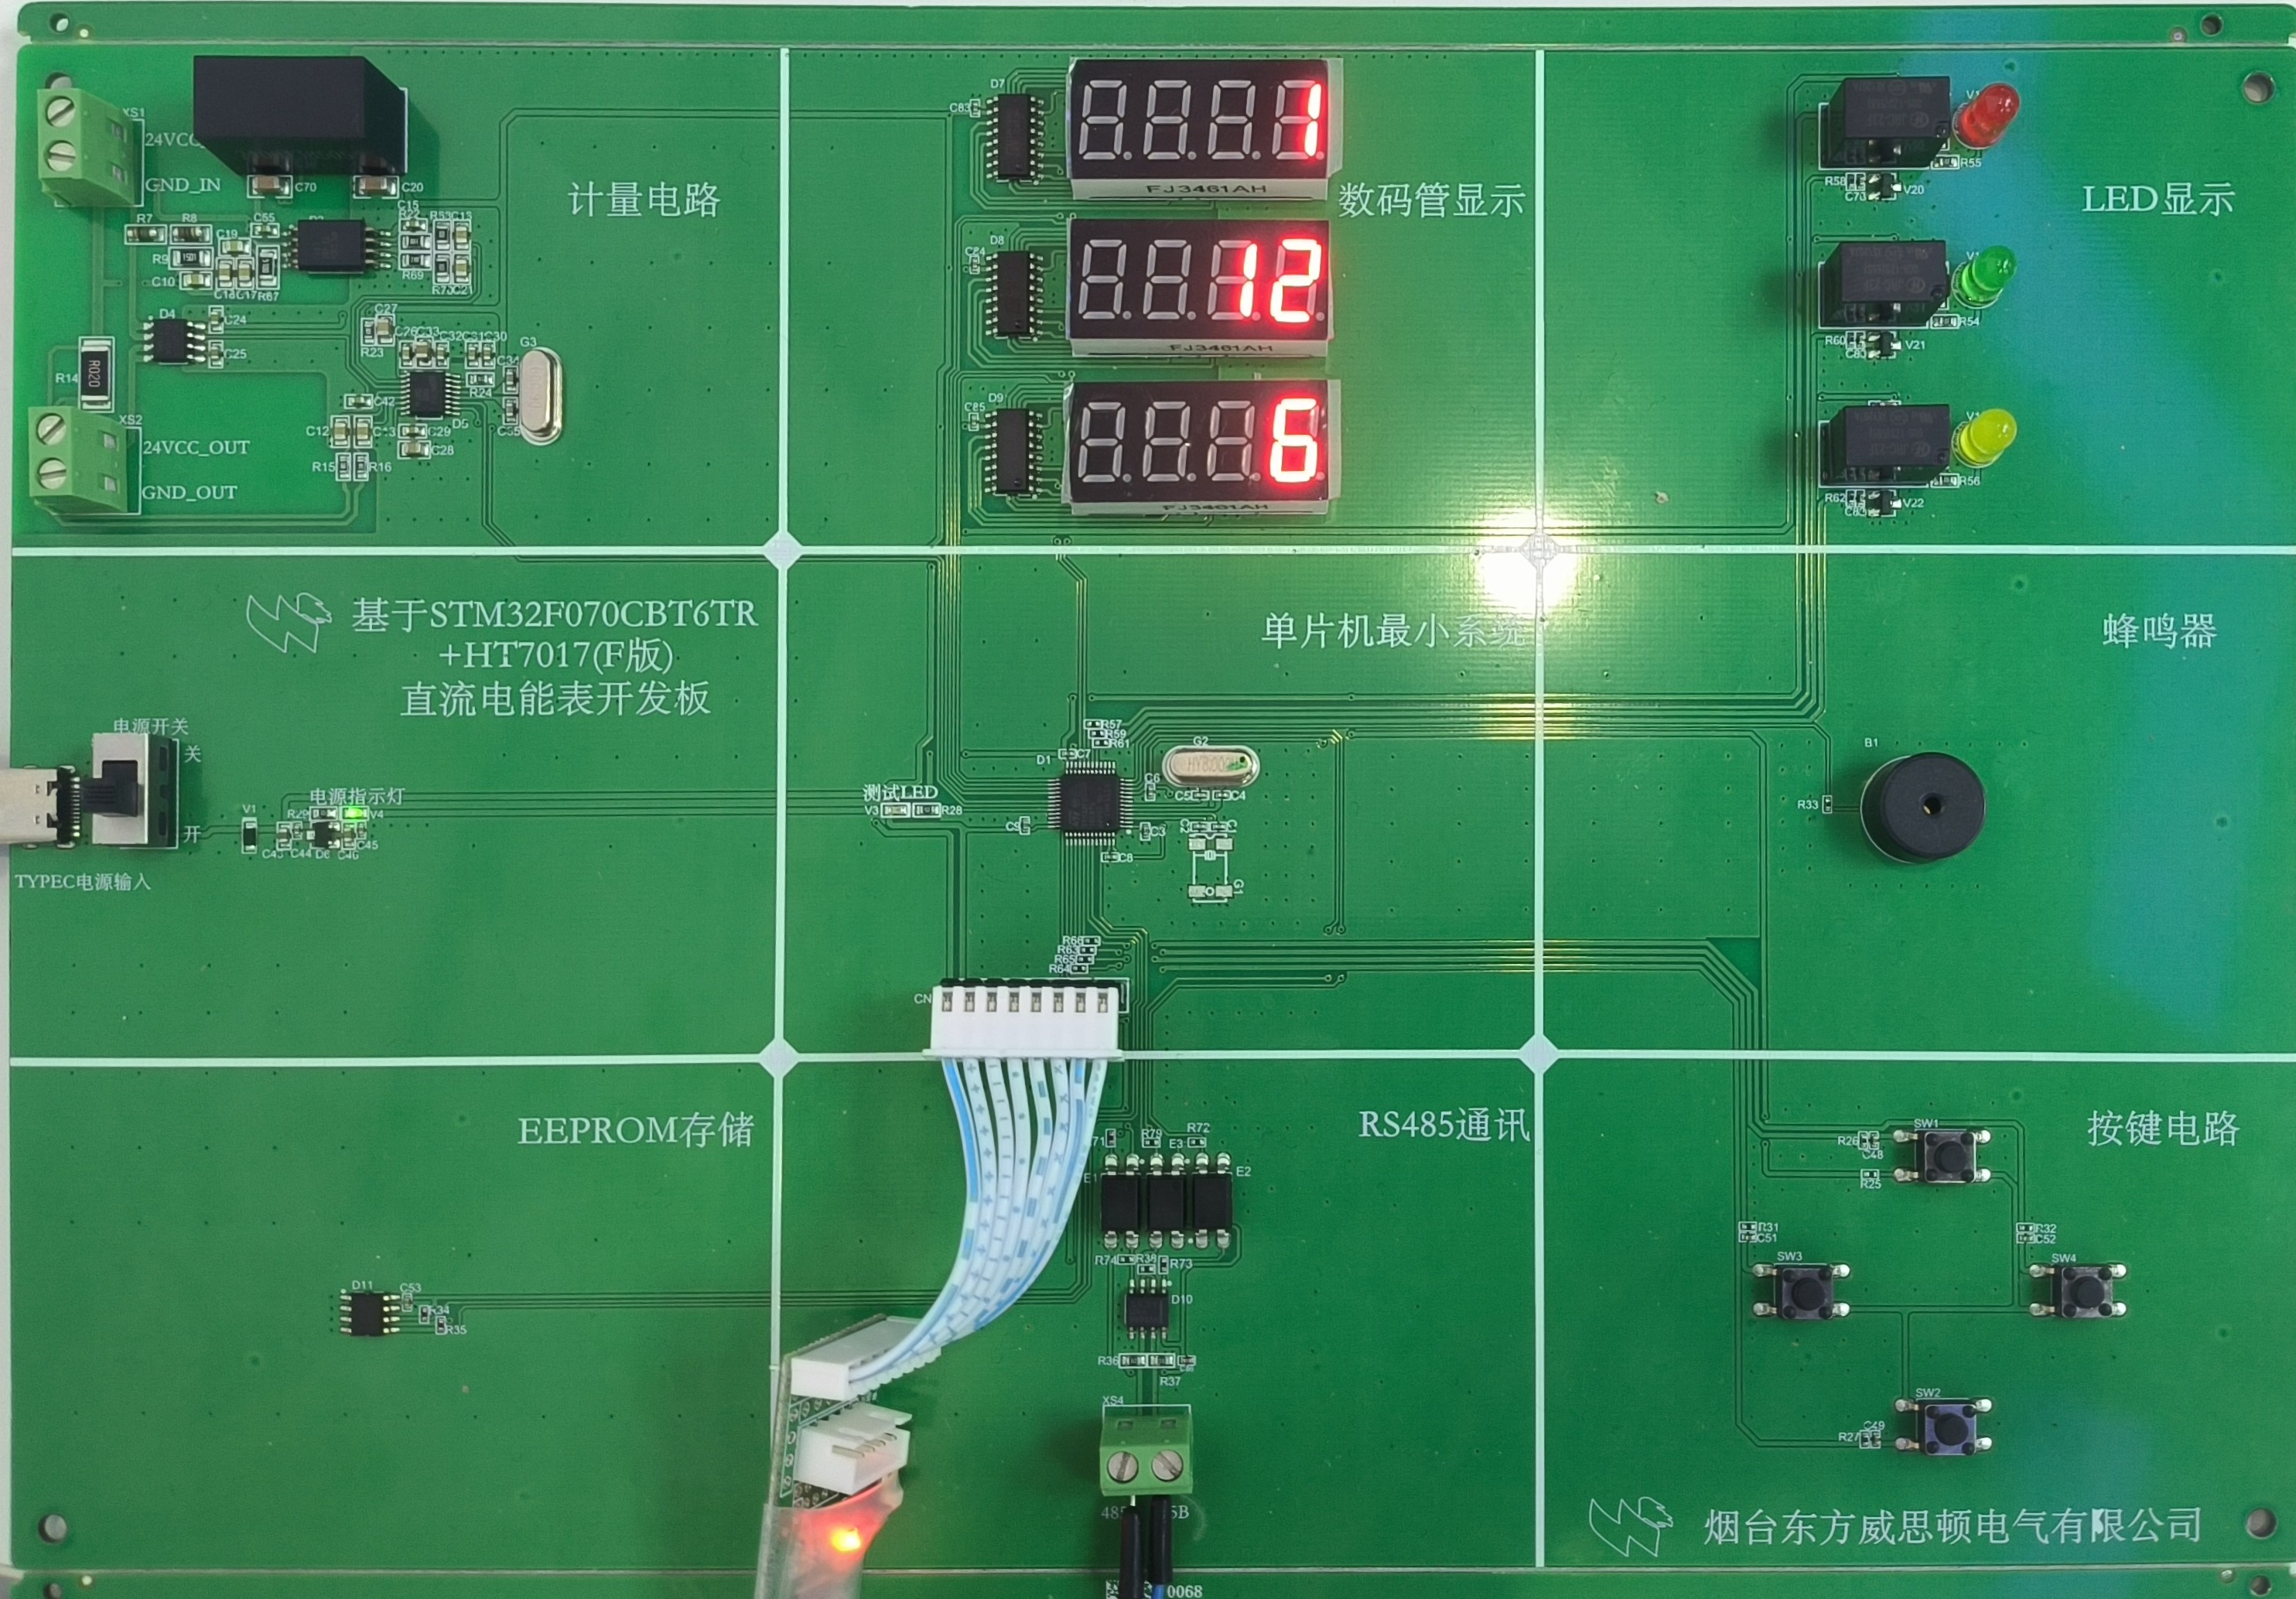
\includegraphics[width=\textwidth]{figs/trafficlight/idle.jpg}
    \caption{红绿灯——初始运行状态}\label{fig:trafficlight/idle.jpg}
  \end{minipage}\hfill
  \begin{minipage}[t]{0.48\textwidth}
    \centering
    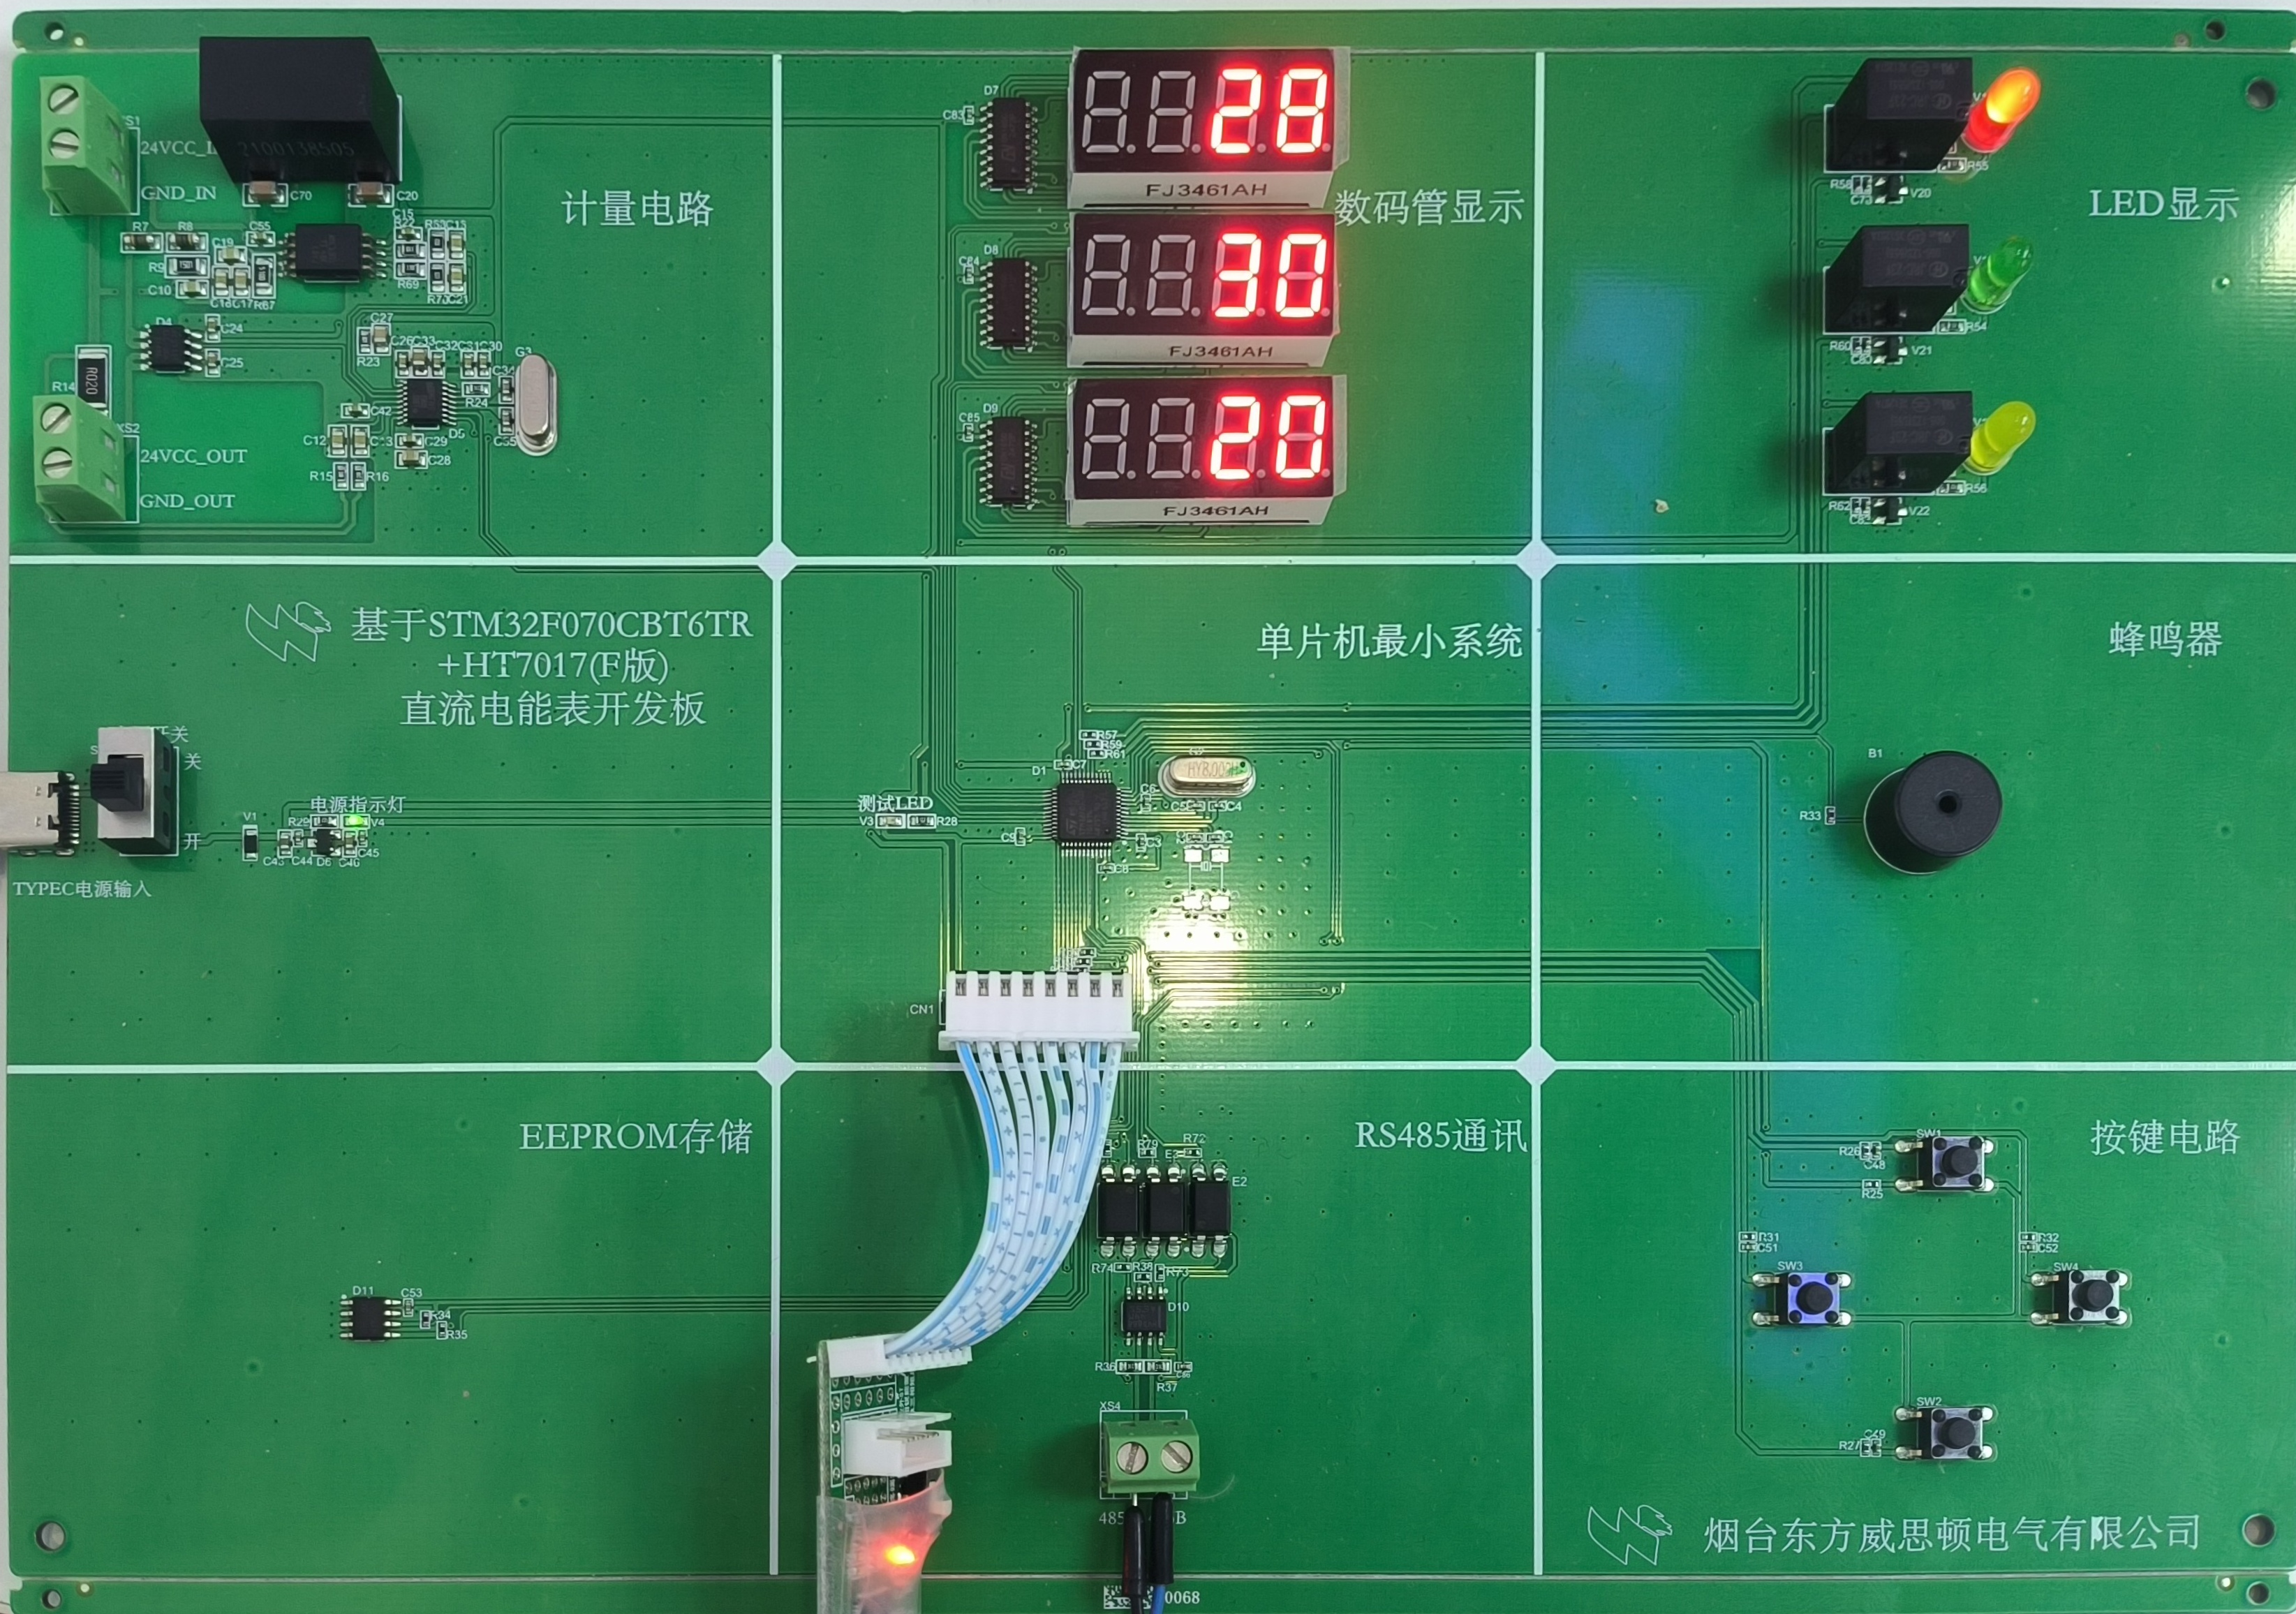
\includegraphics[width=\textwidth]{figs/trafficlight/red_on.jpg}
    \caption{红绿灯——红灯倒计时}\label{fig:trafficlight/red_on.jpg}
  \end{minipage}
\end{figure}

\begin{figure}[H]
  \centering
  \begin{minipage}[t]{0.48\textwidth}
    \centering
    \includegraphics[width=\textwidth]{figs/trafficlight/green_on.jpg}
    \caption{红绿灯——绿灯倒计时}\label{fig:trafficlight/green_on.jpg}
  \end{minipage}\hfill
  \begin{minipage}[t]{0.48\textwidth}
    \centering
    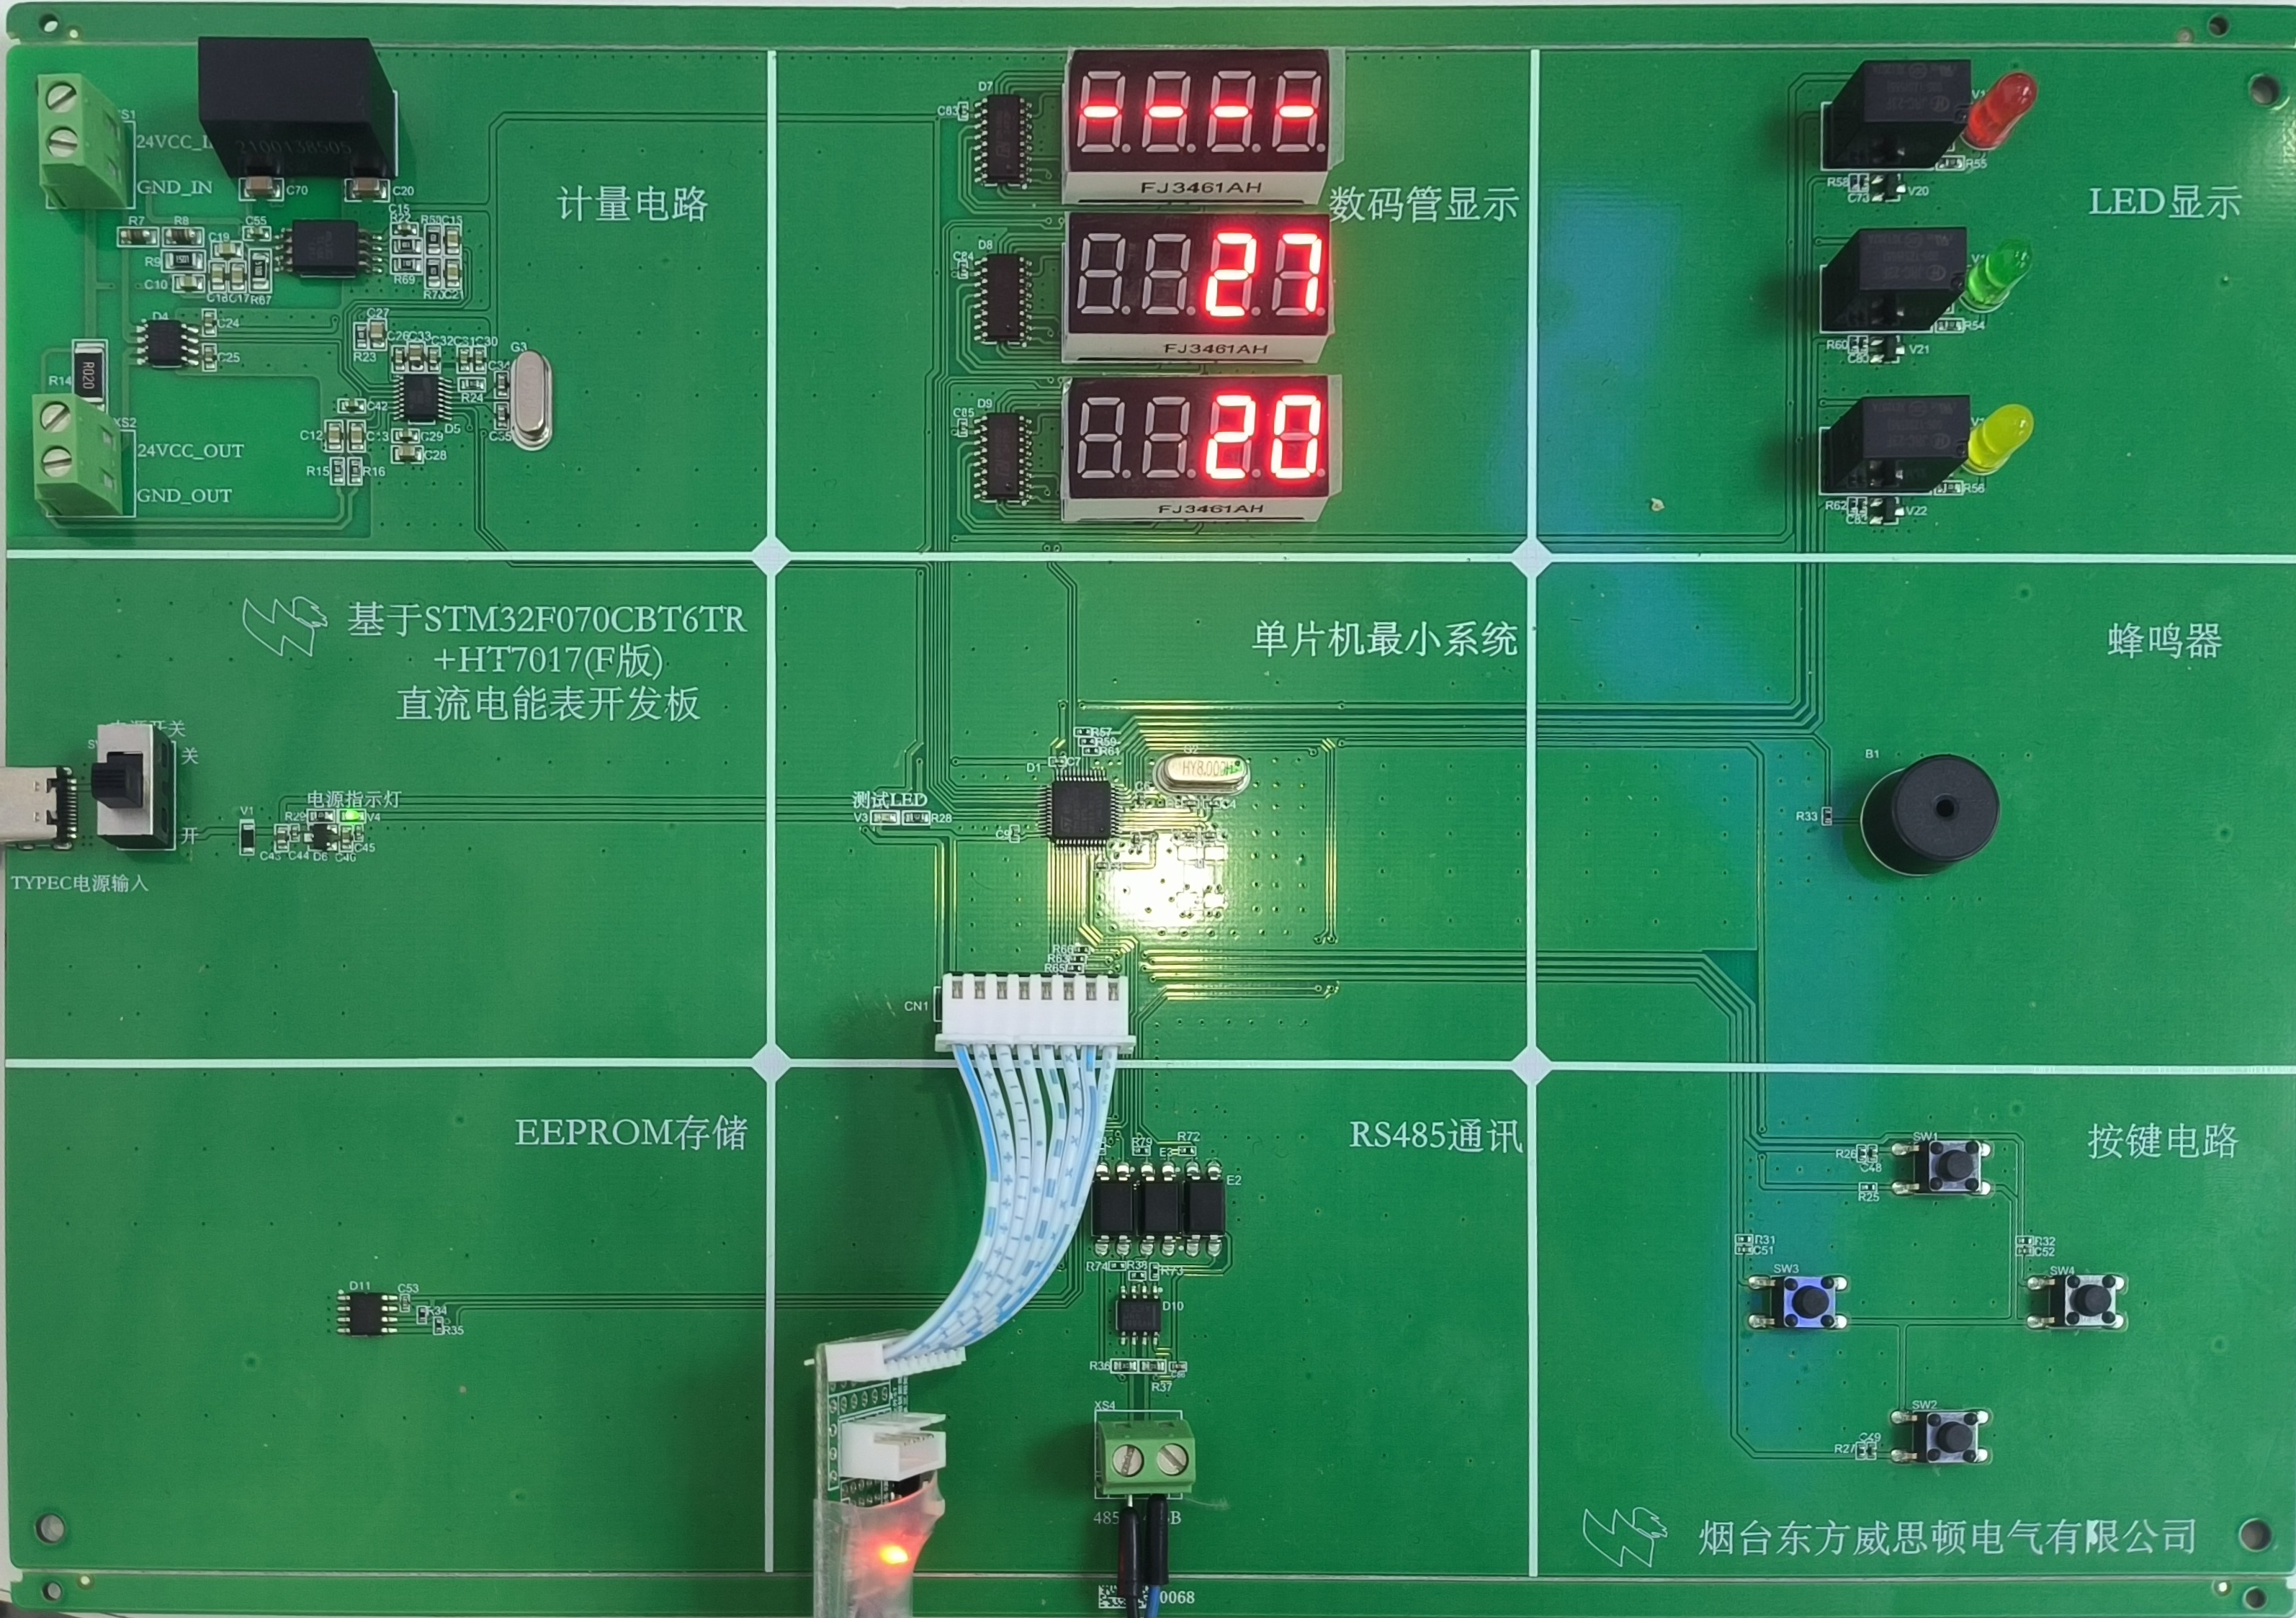
\includegraphics[width=\textwidth]{figs/trafficlight/red_time_set.jpg}
    \caption{红绿灯——设置红灯时长}\label{fig:trafficlight/red_time_set.jpg}
  \end{minipage}
\end{figure}

\insertfigure{0.62}{trafficlight/green_time_set.jpg}{红绿灯——设置绿灯时长}

\subsubsection*{2. 模拟电梯系统}

电梯系统的 8 状态 FSM 运行稳定。按键选择楼层时数码管会闪烁提示；确认后电梯按楼层逐步移动，到达时蜂鸣器短鸣、LED 颜色正确切换，开门等待 3 秒后自动进入下一状态，任务完成后返回 1 楼。全程采用非阻塞方式运行，数码管能够实时更新当前楼层。图~\ref{fig:elevator/begin.jpg} 至图~\ref{fig:elevator/arrived_seg_3.jpg} 展示了电梯系统各阶段的运行状态。

\begin{figure}[H]
  \centering
  \begin{minipage}[t]{0.48\textwidth}
    \centering
    \includegraphics[width=\textwidth]{figs/elevator/begin.jpg}
    \caption{电梯——1 楼待机}\label{fig:elevator/begin.jpg}
  \end{minipage}\hfill
  \begin{minipage}[t]{0.48\textwidth}
    \centering
    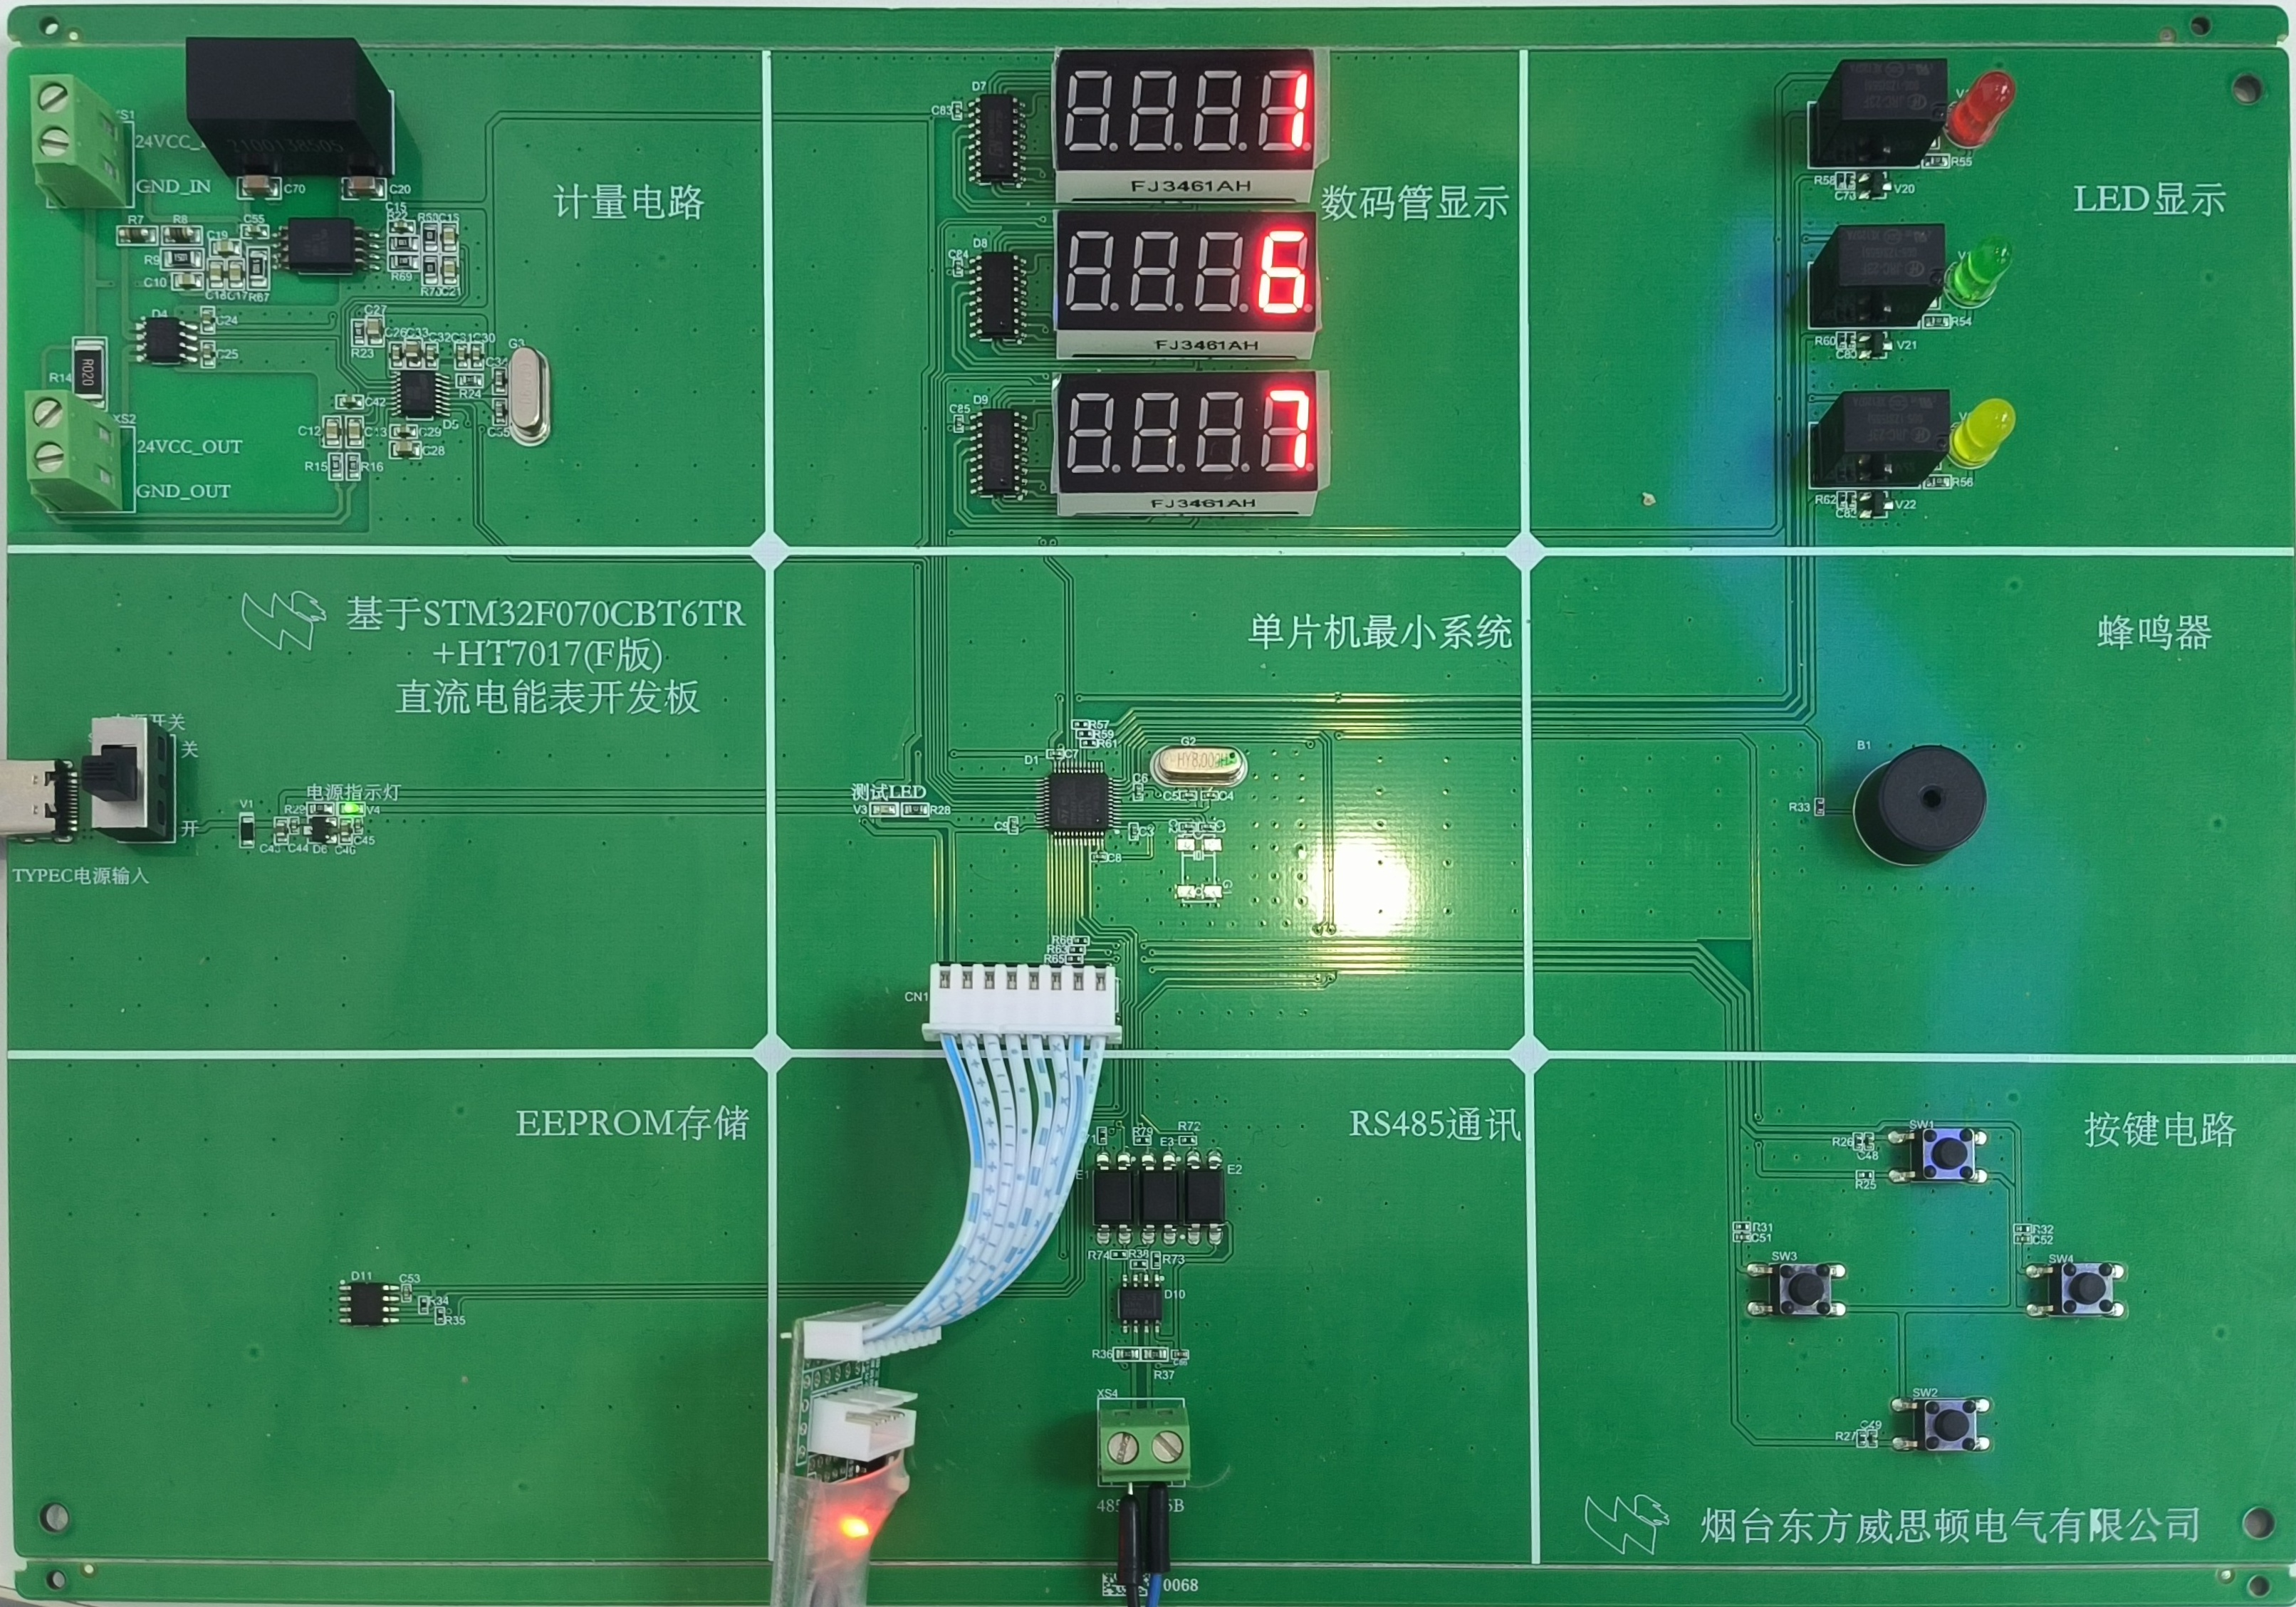
\includegraphics[width=\textwidth]{figs/elevator/set_seg_2.jpg}
    \caption{电梯——选择起始楼层}\label{fig:elevator/set_seg_2.jpg}
  \end{minipage}
\end{figure}

\begin{figure}[H]
  \centering
  \begin{minipage}[t]{0.48\textwidth}
    \centering
    \includegraphics[width=\textwidth]{figs/elevator/set_seg_3.jpg}
    \caption{电梯——选择目标楼层}\label{fig:elevator/set_seg_3.jpg}
  \end{minipage}\hfill
  \begin{minipage}[t]{0.48\textwidth}
    \centering
    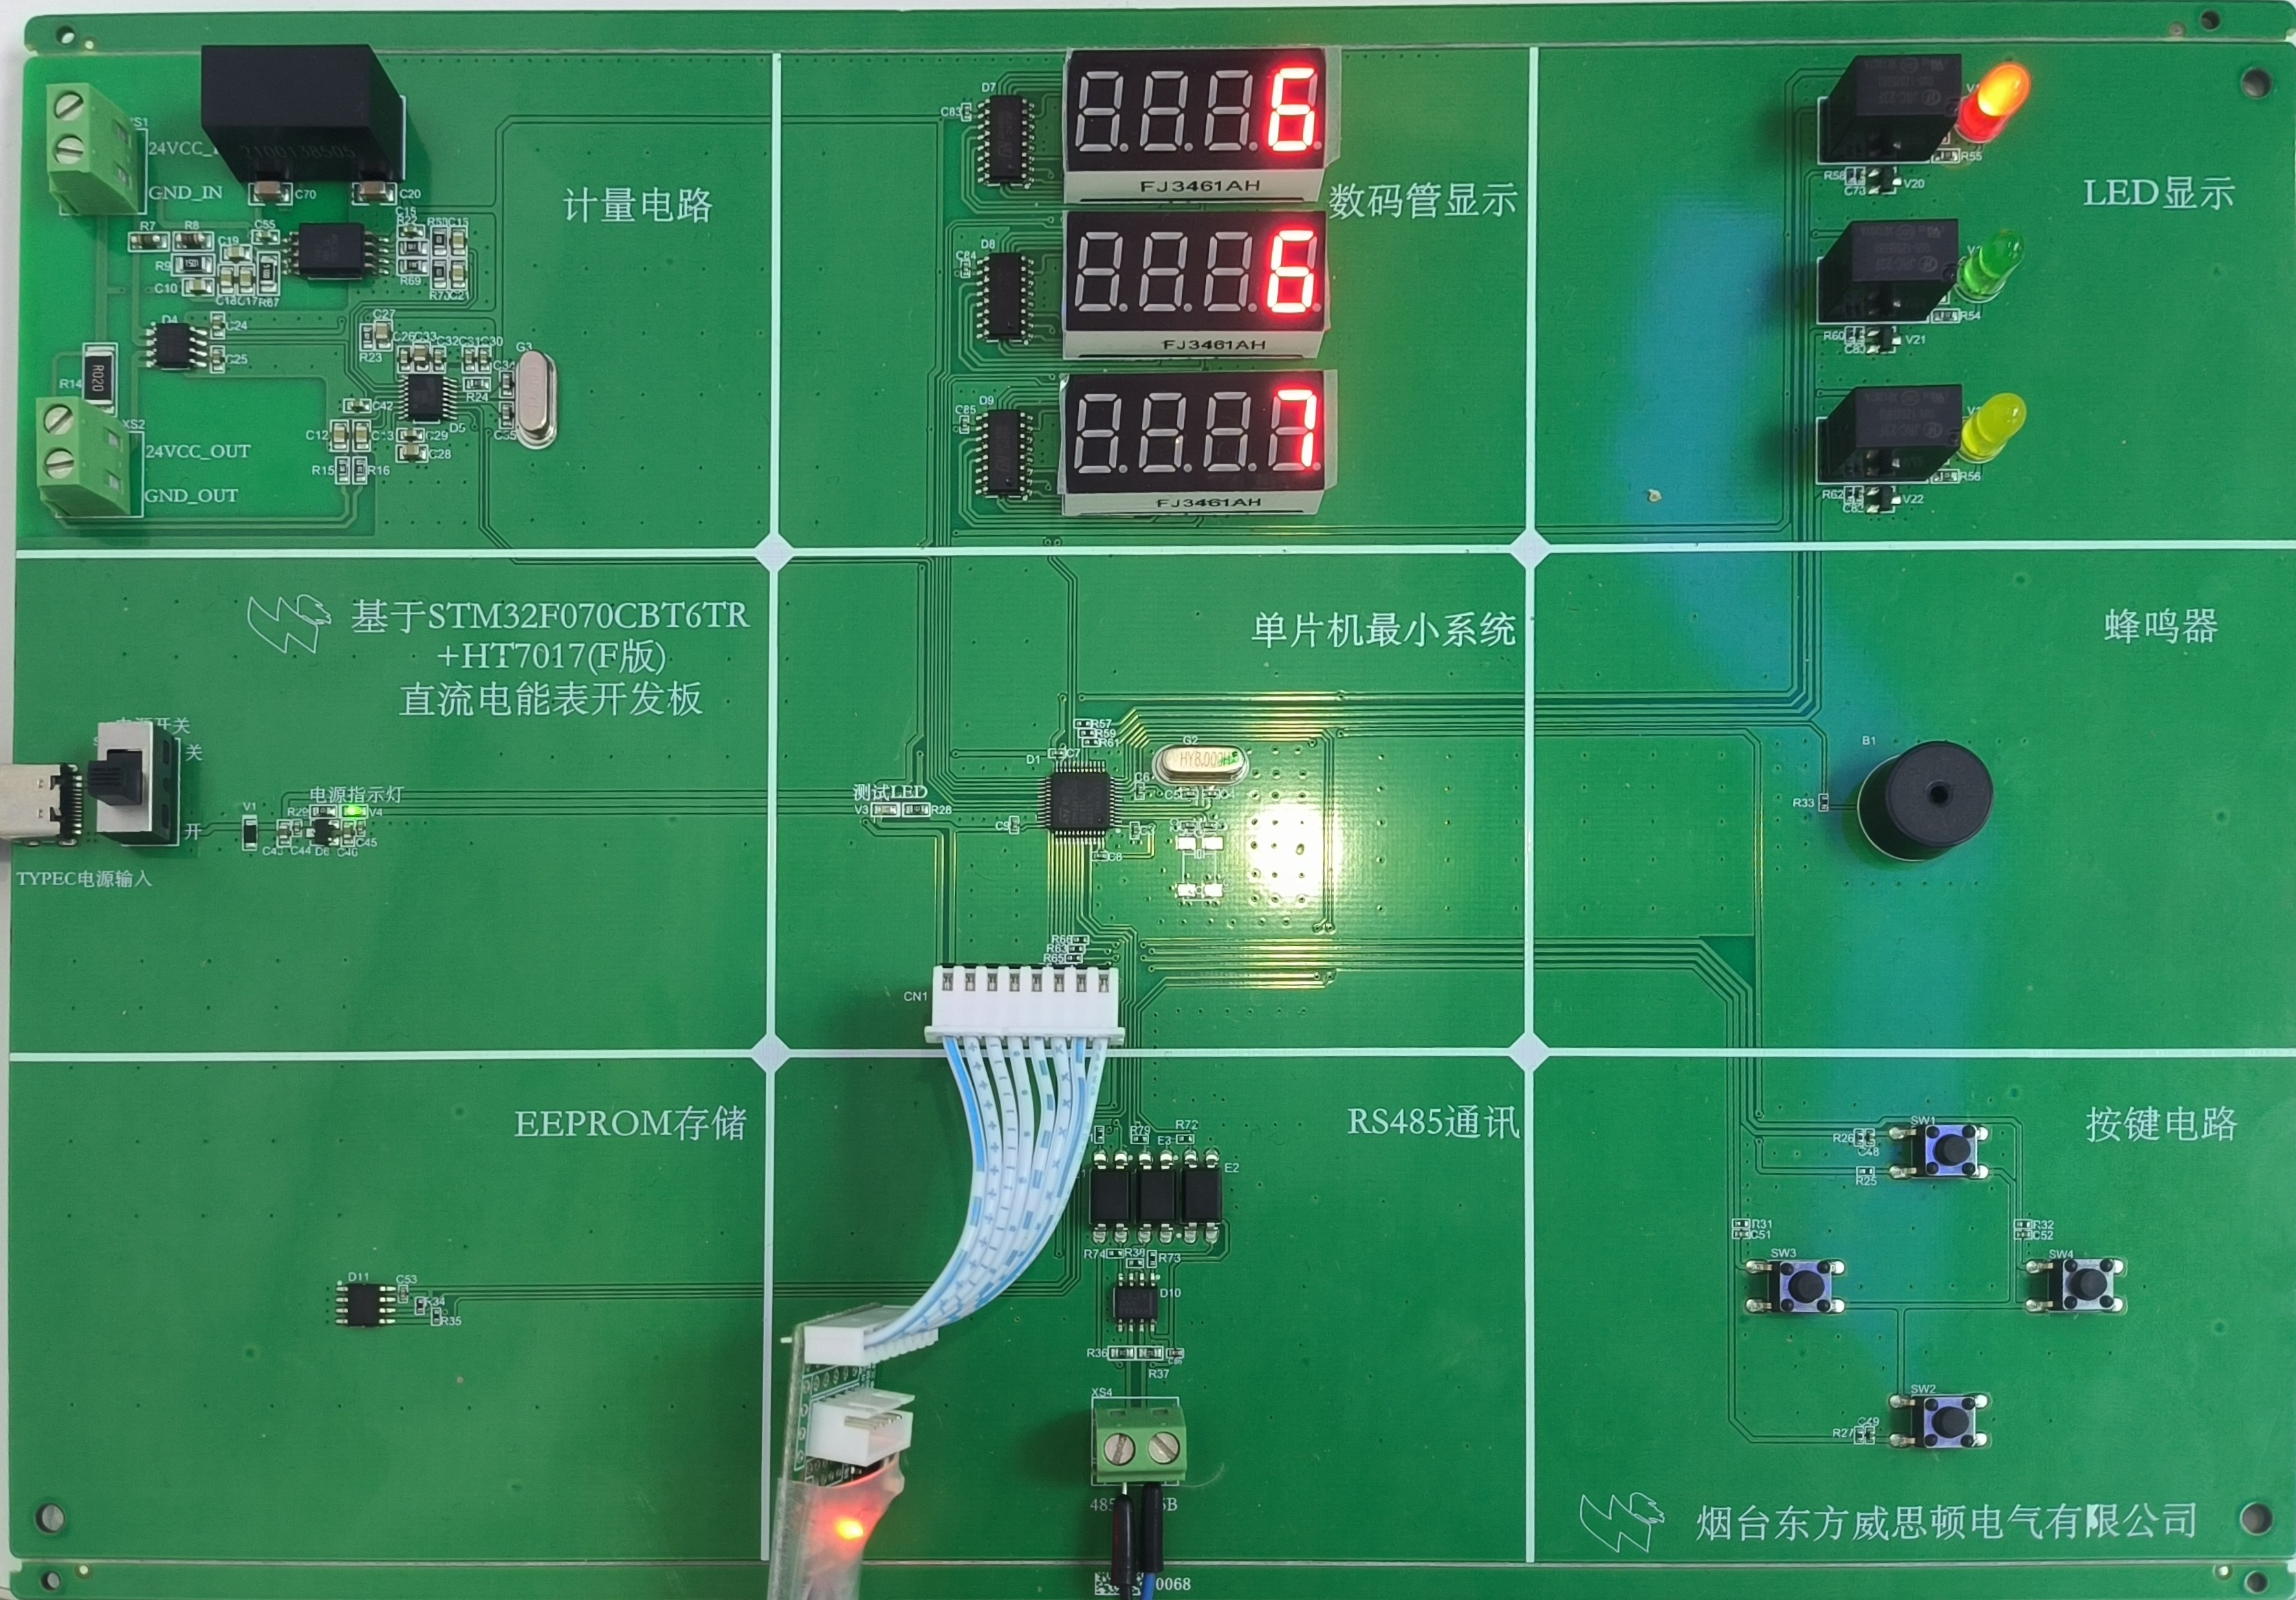
\includegraphics[width=\textwidth]{figs/elevator/running.jpg}
    \caption{电梯——运行中}\label{fig:elevator/running.jpg}
  \end{minipage}
\end{figure}

\insertfigure{0.48}{elevator/arrived_seg_3.jpg}{电梯——到达目标楼层}

\subsubsection*{3. 直流电表数据采集}

HT7017 初始化顺利完成，系统可周期性读取电压、电流和功率的 24 位原始采样值，并在数码管上实时显示；RS485 也能够将数据稳定发送至上位机串口助手。由于实验环境缺少外部 24\,V 负载，采样值接近零或表现为底噪属于正常现象，这表明通信链路与基础采样流程工作正常。图~\ref{fig:energymeter/running.jpg} 和图~\ref{fig:energymeter/uart_log.png} 分别展示了电表运行状态和串口接收数据。

\begin{figure}[H]
  \centering
  \begin{minipage}[t]{0.48\textwidth}
    \centering
    
\includegraphics[width=\textwidth]{figs/energymeter/running.jpg}
    \caption{电表——数码管显示采样值}\label{fig:energymeter/running.jpg}
  \end{minipage}\hfill
  \begin{minipage}[t]{0.48\textwidth}
    \centering
    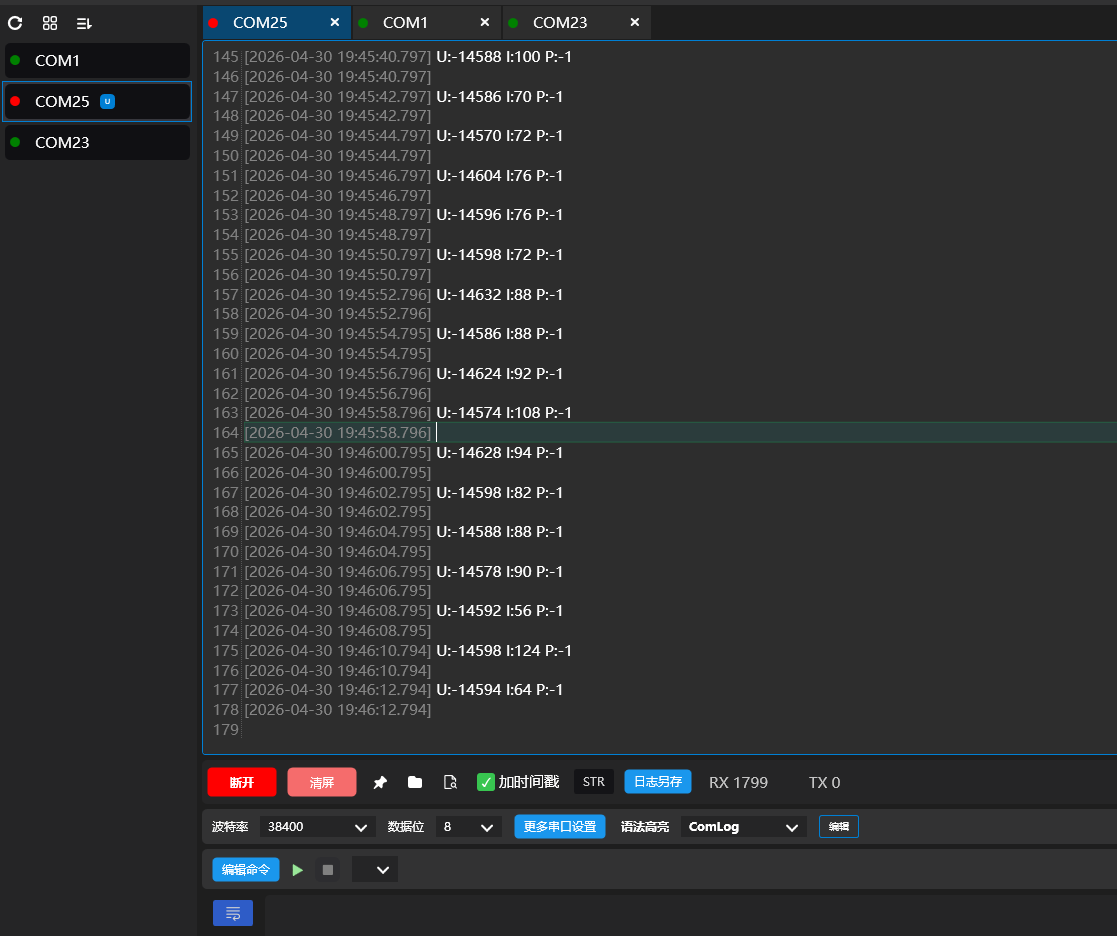
\includegraphics[width=\textwidth]{figs/energymeter/uart_log.png}
    \caption{电表——RS485 串口接收数据}\label{fig:energymeter/uart_log.png}
  \end{minipage}
\end{figure}

% ========== 实验总结与体会 ==========
\section{实验总结与体会}

本次实验完成了红绿灯控制、模拟电梯和直流电表数据采集三个功能模块的开发，使我对嵌入式系统设计流程有了更系统的理解。

主要收获体现在三个方面。第一，通过红绿灯和电梯两个项目掌握了 FSM 在嵌入式系统中的实际应用方法。将状态转移集中在定时器中断中、将 UI 刷新放在主循环中的架构，使代码结构更清晰，也更便于扩展，电梯系统的 8 状态机尤其体现了这一点。第二，电梯系统用定时器中断配合计数器替代 \texttt{HAL\_Delay()} 的非阻塞设计，让我进一步认识到实时系统中应尽量避免空转等待。第三，多协议通信的实践加深了我对嵌入式通信底层实现的理解，尤其是 HT7017 的 9 位数据位奇校验串口配置和 GN1650 的 bit-bang I2C 协议，体现了不同外设对通信参数的差异化需求。

\begin{sloppypar}
实验中还遇到了两个印象深刻的硬件问题。第一个是 RS485 通信始终失败。排查软件配置和通信协议均无异常后，最终发现原因出在上位机链路接线方式判断错误：实验中开发板 PCB 先接入 ``野火小智'' 模块，再由该模块接入 CH340(HW597) 串口模块。这一路径属于普通串口通信，``野火小智'' 与 CH340(HW597) 的正确连接应为 TX 对 TX、RX 对 RX；而 HC-05 蓝牙模块才采用 TX 对 RX、RX 对 TX 的交叉连接方式。实验中误把 RS485 链路也按蓝牙方式接成了交叉连接，导致通信一直失败。这一错误耗费了大量调试时间，也提醒我在排查通信故障时必须先确认链路拓扑与接口类型，再决定接线方式。第二个问题出现在实验室机房环境中。由于串口线较短，我将开发板直接放置在台式机金属机箱上，导致 \texttt{HAL\_Init()} 执行失败，程序无法正常启动。分析原因是金属机箱作为导体，使开发板底部裸露焊点与机箱之间形成了意外电气连接，干扰了芯片的正常初始化。将开发板移至绝缘桌面后，问题立即消失。这两个问题虽然都不涉及复杂的软件调试，却让我更加明确地认识到嵌入式开发中硬件环境和物理连接的重要性，不少所谓的``软件问题''根源其实在硬件层面。
\end{sloppypar}

\end{document}
